
\documentclass{article}
\usepackage[utf8]{inputenc}
\usepackage{graphicx}
\usepackage{subcaption}
\usepackage{tikz} 
 \usetikzlibrary{arrows,automata,positioning,petri}
 
\title{Report on Labwork 6}
\author{TRAN Thi Hong Hanh}

\begin{document}

\maketitle
\section{Explain how you implement the labwork?}
\begin{verbatim}
//Initialize extra parameters for labwork 6
        int option;
        option = atoi(argv[3]);
        float timeBinarize, timeBright, timeBlend;
        int parama, paramb;
        float paramc;

        switch (option)
        {
        case 0:
            parama = atoi(argv[4]);
            timer.start();
            labwork.labwork6a_GPU(parama);
            timeBinarize = timer.getElapsedTimeInMilliSec();

            labwork.saveOutputImage("labwork6a-gpu-out.jpg");
            printf("Labwork 6a (Binarization) ellapsed %.1fms\n", lwNum, timeBinarize);
            break;
        case 1:
            paramb = atoi(argv[4]);
            timer.start();
            labwork.labwork6b_GPU(paramb);
            timeBright = timer.getElapsedTimeInMilliSec();

            printf("Labwork 6b (Brightness) ellapsed %.1fms\n", lwNum, timeBright);
            labwork.saveOutputImage("labwork6b-gpu-out.jpg");
            break;
        case 2:
            paramc = atof(argv[4]);
            std::string inputFilename1;
            JpegInfo *inputImage1;

            inputFilename1 = std::string(argv[5]);
            inputImage1 = labwork.loadImage(inputFilename1);

            timer.start();
            labwork.labwork6c_GPU(paramc, inputImage1);
            timeBlend = timer.getElapsedTimeInMilliSec();

            printf("Labwork 6c (Blending) ellapsed %.1fms\n", lwNum, timeBlend);
            labwork.saveOutputImage("labwork6c-gpu-out.jpg");
            break;
        }
        break;
\end{verbatim}
\subsection{6a: Binarization}
\begin{itemize}
    \item Add an extra parameter from the command line for threshold using \textbf{argv}.
    \item Convert a greyscale pixel to binary one based on the threshold.
    \begin{verbatim}
    unsigned char binary = (input[tid].x + input[tid].y + input[tid].z) / 3;
    binary = min(binary / thres, 1) * 255;
    \end{verbatim}
    \item Command:
    \begin{verbatim}
        ./labwork 6 ../data/cloud.jpeg 0 127 
    \end{verbatim}
    \item Result:
    \begin{verbatim}
    USTH ICT Master 2019, Advanced Programming for HPC.
    Warming up...
    Starting labwork 6
    Labwork 6a (Binarization) ellapsed 15.9ms
    Labwork 6 ellapsed 23.3ms
    \end{verbatim}
    \begin{figure}[h]
      \centering
      \begin{subfigure}{.45\textwidth}
        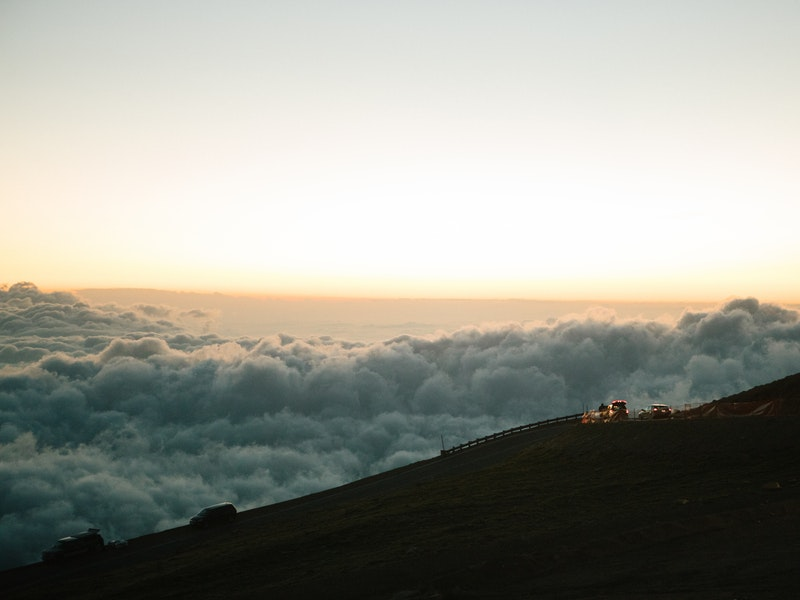
\includegraphics[width=\linewidth]{./result/cloud.jpeg}
        \caption{Original image}
      \end{subfigure}
      \hspace{1cm}
      \begin{subfigure}{.45\textwidth}
        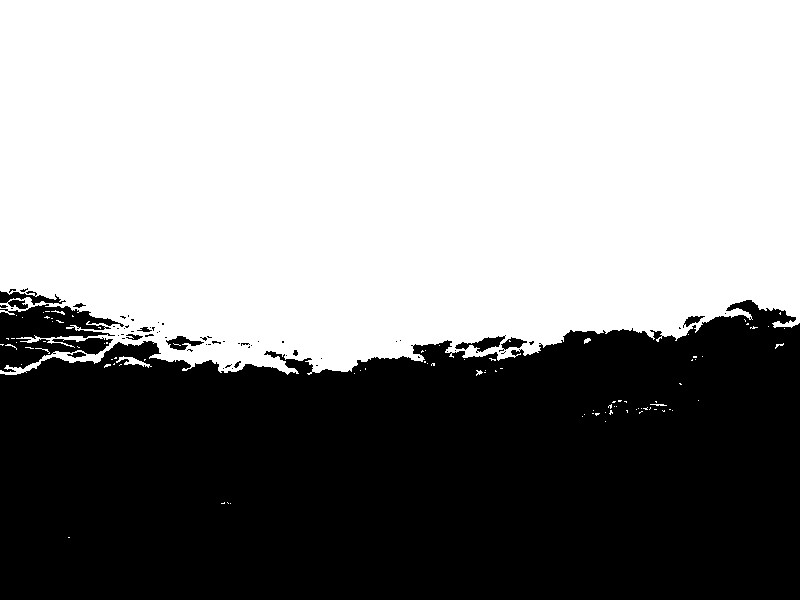
\includegraphics[width=\linewidth]{./result/labwork6a-gpu-out.jpg}
        \caption{Binarization using threshold of 127}
      \end{subfigure}
    \end{figure}
\end{itemize}
\newpage
\subsection{6b: Brightness control}
\begin{itemize}
    \item Add an extra parameter from the command line for brightness using \textbf{argv}.
    \item Use max/min method avoid the changes that exceed the range of color's value.
    \begin{verbatim}
    unsigned char red = min(max(input[tid].x + brightness, 0), 255);
    unsigned char green = min(max(input[tid].y + brightness, 0), 255);
    unsigned char blue = min(max(input[tid].z + brightness, 0), 255);
    \end{verbatim}
    \item Command:
    \begin{verbatim}
        ./labwork 6 ../data/cloud.jpeg 1 100
    \end{verbatim}
    \item Result:
    \begin{verbatim}
    USTH ICT Master 2019, Advanced Programming for HPC.
    Warming up...
    Starting labwork 6
    Labwork 6b (Brightness) ellapsed 31.9ms
    Labwork 6 ellapsed 54.4ms
    \end{verbatim}
    \begin{figure}[h]
      \centering
      \begin{subfigure}{.45\textwidth}
        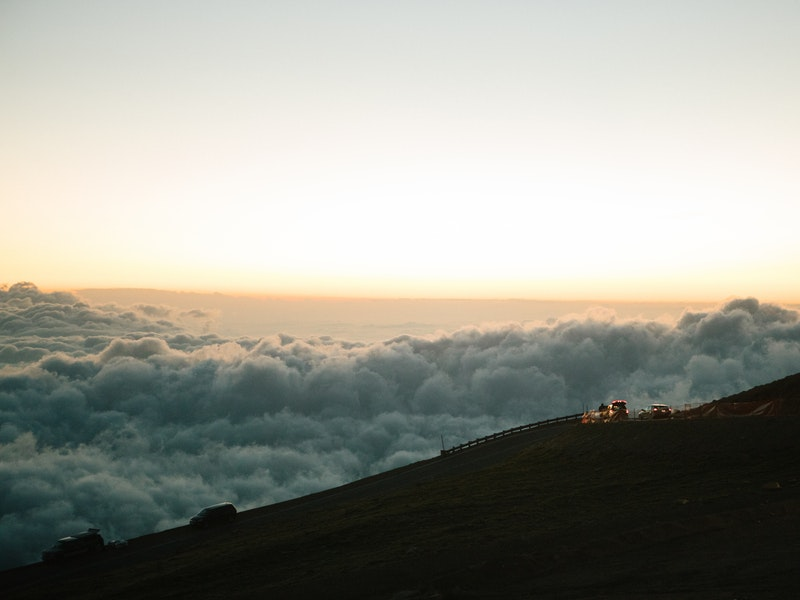
\includegraphics[width=\linewidth]{./result/cloud.jpeg}
        \caption{Original image}
      \end{subfigure}
      \hspace{1cm}
      \begin{subfigure}{.45\textwidth}
        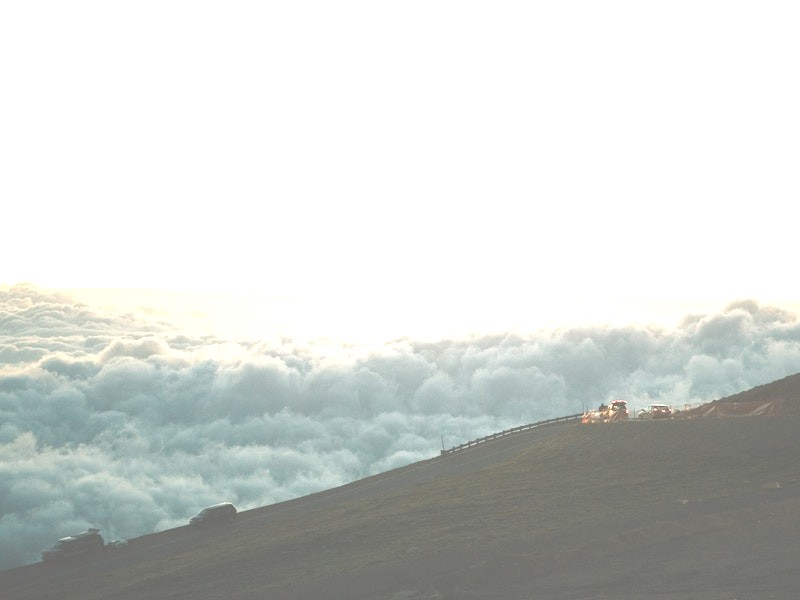
\includegraphics[width=\linewidth]{./result/labwork6b-gpu-out.jpg}
        \caption{Brightness = 100}
      \end{subfigure}
    \end{figure}
\end{itemize}
\subsection{6c: Blending images }
\begin{itemize}
    \item Add an extra parameter from the command line for blending ratio using \textbf{argv}.
    \item Compute the average pixel's colors between two images by the ratio.
    \begin{verbatim}
unsigned char red = input[tid].x * blendRatio + input1[tid].x * (1 - blendRatio);
unsigned char green = input[tid].y * blendRatio + input1[tid].y * (1 - blendRatio);
unsigned char blue = input[tid].z * blendRatio + input1[tid].z * (1 - blendRatio);
    \end{verbatim}
    \item Command:
    \begin{verbatim}
        ./labwork 6 ../data/cloud.jpeg 2 0.5 ../data/leaf.jpg 
    \end{verbatim}
    \item Result:
    \begin{verbatim}
    USTH ICT Master 2019, Advanced Programming for HPC.
    Warming up...
    Starting labwork 6
    Labwork 6c (Blending) ellapsed 14.5ms
    Labwork 6 ellapsed 46.9ms
    \end{verbatim}
    \begin{figure}[h]
      \centering
      \begin{subfigure}{.45\textwidth}
        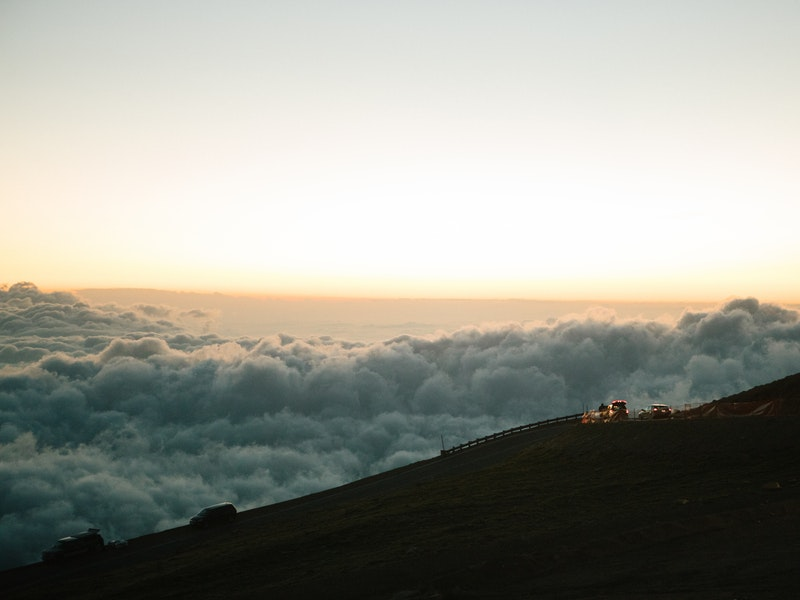
\includegraphics[width=\linewidth]{./result/cloud.jpeg}
        \caption{Original image}
      \end{subfigure}
      \hspace{1cm}
      \begin{subfigure}{.45\textwidth}
        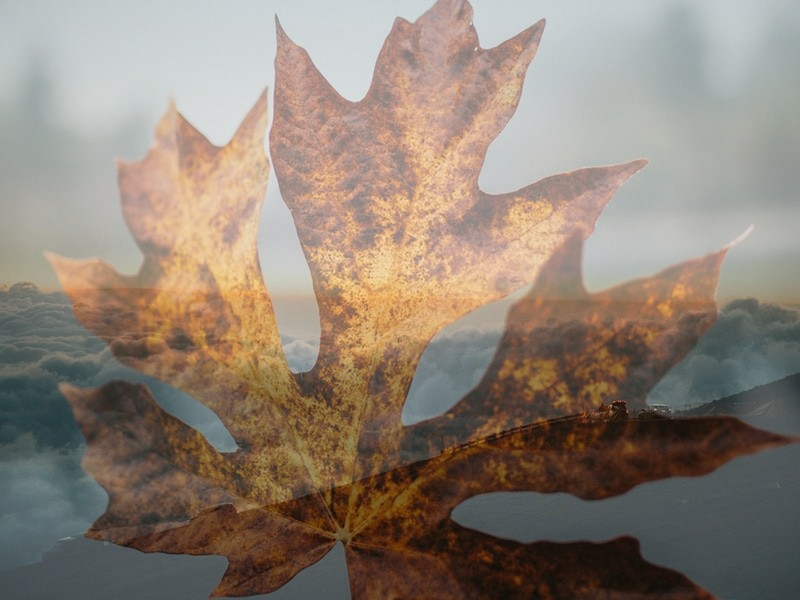
\includegraphics[width=\linewidth]{./result/labwork6c-gpu-out.jpg}
        \caption{Blending using ratio of 0.5}
      \end{subfigure}
    \end{figure}
\end{itemize}

\end{document}
